\section{Techniken des Inductive Logic Programming}
\frame{\frametitle{Agenda}\tableofcontents[currentsection]}
\subsection{Finden des Hypothesenraums}
\begin{frame}
	\frametitle{Subsumption von Literalen}
	\emph{Idee}: Eingrenzung des Suchraums erleichtert Hypothesensuche

	\begin{block}{Definition: Subsumption für Literale/Atome}
		Seien $L_1$ und $L_2$ Literale: $L_1 \underbrace{\preceq}_{\text{subsumiert}} L_2$
		wenn eine Substitution $\theta$ existert, sodass:
		\begin{align*}
			 L_1 \theta \subseteq L_2
		\end{align*}
	\end{block}
	\begin{bsp}
		\begin{align*}
			 daughter(X, Y)\theta\subseteq daughter(mary, ann)\\\text{  mit  } \theta = \{X/mary, Y/ann\}
		\end{align*}
	\end{bsp}
\end{frame}
\begin{frame}
	\frametitle{Subsumption von Klauseln}
	Das gleiche Prozedere für Klauseln:
	\begin{block}{Definition: Subsumption für Klauseln}
		Seien $C_1$ und $C_2$ Klauseln: $C_1 \underbrace{\preceq}_{\text{subsumiert}} C_2$
		wenn eine Substitution $\theta$ existert, sodass:
		\begin{align*}
			 C_1 \theta \subseteq C_2
		\end{align*}
	\end{block}
	\begin{bsp}
		\begin{align*}
			(daughter(X, Y)      &\leftarrow parent(Y,X))\theta \subseteq\\
			 daughter(mary, ann) &\leftarrow female(mary), parent(ann, mary),\\
			                     & parent(tom, mary)\\
			 \text{  mit  } \theta = \{X/mary, Y/ann\}
		\end{align*}
	\end{bsp}
\end{frame}

\begin{frame}
	\frametitle{Eigenschaften der Subsumption}
	\begin{enumerate}
		\item {
			Wenn $C_1 \preceq C_2$ dann gilt (nicht umgekehrt!):
			\begin{align*}
				C_1 \vDash C_2
			\end{align*}
		}
		\item{ Die Relation $\preceq$ führt ein Gitter (lattice) von reduzierten Klauseln ein
			\begin{figure}[H]
				\begin{center}
					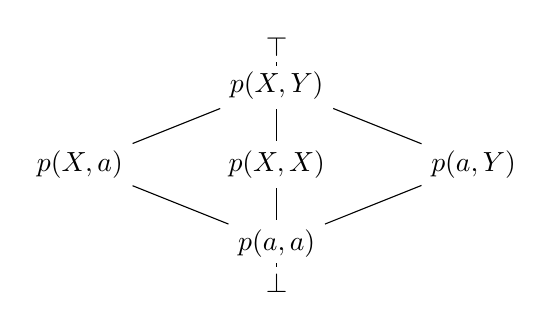
\begin{tikzpicture}
						\node (G) at (1.5,2) {$\top$};
						\node (A) at (1.5,1.5) {$p(X,Y)$};
						\node (B) at (-1,0.5) {$p(X,a)$};
						\node (C) at (1.5,0.5) {$p(X,X)$};
						\node (D) at (4,0.5) {$p(a,Y)$};
						\node (E) at (1.5,-0.5) {$p(a,a)$};
						\node (F) at (1.5,-1) {$\bot$};
			
						\path [-] (A) edge node[left] {} (G);
						\path [-] (A) edge node[left] {} (B);
						\path [-] (A) edge node[left] {} (C);
						\path [-] (A) edge node[left] {} (D);
						\path [-] (B) edge node[left] {} (E);
						\path [-] (C) edge node[left] {} (E);
						\path [-] (D) edge node[left] {} (E);
						\path [-] (F) edge node[left] {} (E);
					\end{tikzpicture}
				\end{center}
				\caption{Partiell geordnete Menge von Formeln (POSET)}
				\label{fig:poset_atomic}
			\end{figure}
		}
	\end{enumerate}
\end{frame}

\subsection{Bottom-up -- Least general generalization}
\begin{frame}
	\frametitle{Bottom-up -- Least general generalization (LGG)}
	 Die \textit{least general generalization} von zwei Klauseln $C_1, C_2$ ist
	 die kleinste obere Schranke von $C_1,C_2$ im Gitter.

	\begin{block}{Erkenntnisse}
			\begin{itemize}
				\item [$\Rightarrow$] Alle Beispiele die $C_1$ abdeckt werden auch von
				allen 'kleineren Klauseln' abgedeckt
				\item[$\Rightarrow$] Wenn $C_1$ ein Beispiel nicht abdeckt,
				dann tut dies auch keine 'kleinere Klausel'
			\end{itemize}
	 \end{block}
\end{frame}

\begin{frame}
	\frametitle{Bottom-up -- Least general generalization (LGG)}
	\begin{block}{$lgg$ von Termen}
		\begin{enumerate}
			\item $lgg(t,t) = t$\\
			\item $lgg(f(s_1, \ldots, s_n), f(t_1, \ldots, t_n)) = f(lgg(s_1, t_1), \ldots, lgg(s_n, t_n))$
			\item Sonst: $lgg(t_1, t_2) = v , v$ freie Variable
		\end{enumerate}
	\end{block}
	\begin{block}{$lgg$ von Literalen}
	\begin{enumerate}
		\item $lgg(p(u_1, \ldots, u_n), p(s_1, \ldots, s_n)) = p(lgg(u_1, s_1), \ldots, lgg(u_n, s_n))$\\
		\item Sonst: $lgg(L_1, L_2) = \top$
	\end{enumerate}
	\end{block}
\end{frame}


\begin{frame}
\frametitle{Bottom-up -- Relative least general generalization}
\begin{block}{Definition -- Relative least general generalization}
	Gegeben: Hintergrundwissen $\mathcal{B}$ besteht nur aus \emph{ground literals} (Literale ohne Variablen).
	Sei $K$ die Konjunktion aller Hintergrundliterale und $e_1, e_2$ je positive Beispiele
	\begin{align*}
		rlgg(e_1, e_2) = lgg((e_1 \leftarrow K), (e_2 \leftarrow K))\\
		\Rightarrow \text{ Das Hintergrundwissen wird negiert}
	\end{align*}
\end{block}

\end{frame}


\begin{frame}{Linearity}
\frametitle{Bottom-up -- Relative least general generalization}
	\pgfdeclarelayer{background}
	\pgfsetlayers{background,main}
	\tikzstyle{vertex}=[rectangle,fill=black!25,minimum size=20pt,inner sep=0pt]
	\tikzstyle{selected vertex} = [vertex, fill=red!24]
	\tikzstyle{edge} = [draw,thick,-]
	\tikzstyle{weight} = [font=\small]
	\tikzstyle{selected edge} = [draw,line width=5pt,-,red!50]
	\setbeamercovered{invisible}
	\begin{figure}
		\begin{tikzpicture}[scale=1.0, auto,swap]
		\node[vertex] (a) at (0,0) {$A = e_1 \leftarrow K$};
		\node[vertex] (b) at (2.5,0) {$B = e_2 \leftarrow K$};
		\node[vertex] (c) at (5,0) {$C = e_3 \leftarrow K$};
		\node[vertex] (d) at (7.5,0) {$D = e_4 \leftarrow K$};\pause
		\node[vertex] (e) at (1.25,2) {$C' = lgg(A, B)$};
		\node[vertex] (f) at (6.25,2) {$C''= lgg(C, D)$};\pause
		\node[vertex] (g) at (3.75,4) {$\mathcal{H} = lgg(C', C'')$};
		\begin{pgfonlayer}{background}
			\path<2->[selected edge] (a.center) -- (e.center);
			\path<2->[selected edge] (b.center) -- (e.center);
			\path<2->[selected edge] (c.center) -- (f.center);
			\path<2->[selected edge] (d.center) -- (f.center);
			\path<3->[selected edge] (e.center) -- (g.center);
			\path<3->[selected edge] (f.center) -- (g.center);
		\end{pgfonlayer}
		\end{tikzpicture}
	\end{figure}
\end{frame}

\begin{frame}
	\frametitle{Bottom-up -- Relative least general generalization}
	Beispiel: Familienkonstellation (siehe Terminal)
	\begin{figure}[H]
		\begin{center}
			\begin{tikzpicture}[scale=0.6]
				\node (A) at (0, 2)  {\color{blue}georg};
				\node (B) at (2,0)   {\color{red}mary};
				\node (C) at (4, 2)   {\color{red}ann};
				\node (D) at (6,0)   {\color{blue}tom};
				\node (E) at (8, -2) {\color{red}eve};

				\path [->] (A) edge node[above] {} (B);
				\path [<-] (B) edge node[above] {} (C);
				\path [->] (C) edge node[above] {} (D);
				\path [->] (D) edge node[above] {} (E);
			\end{tikzpicture}
		\end{center}
		\caption{Eine schrecklich nette Famlie}
	\end{figure}
\end{frame}

\begin{frame}
	\frametitle{Bottom-up -- Relative least general generalization}
	\begin{minipage}{0.5\textwidth}
	\begin{block}{Hintergrundwissen der Familienkonstellation}
		\begin{align*}
			K   &= p(a,m), p(a,t), p(t,e),\\ &p(t,i), f(a), f(m), f(e)\\
			e_1 &= daughter(m, a)\\
			e_2 &= daughter(e, t)
		\end{align*}
	\end{block}
	\end{minipage}
	\begin{minipage}{0.45\textwidth}
	\begin{figure}[H]
		\begin{center}
			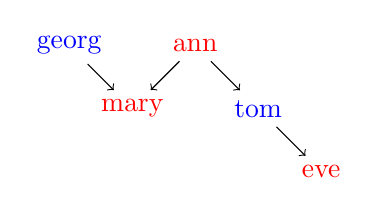
\begin{tikzpicture}[scale=0.4]
				\node (A) at (0, 2)  {\color{blue}georg};
				\node (B) at (2,0)   {\color{red}mary};
				\node (C) at (4, 2)   {\color{red}ann};
				\node (D) at (6,0)   {\color{blue}tom};
				\node (E) at (8, -2) {\color{red}eve};

				\path [->] (A) edge node[above] {} (B);
				\path [<-] (B) edge node[above] {} (C);
				\path [->] (C) edge node[above] {} (D);
				\path [->] (D) edge node[above] {} (E);
			\end{tikzpicture}
		\end{center}
	\end{figure}
	\end{minipage}
	\vspace{8pt}
	\begin{gather*}
		\begin{split}
			\emph{d(V_{m,e}, V_{a,t})} \leftarrow &\; p(a,m), p(a,t), p(t,e), p(t,i), f(a), f(m), f(e),\\
			&\; p(a, V_{m,t}), \emph{p(V_{a,t}, V_{m,e})}, p(V_{a,t}, V_{m,i}), p(V_{a,t}, V_{t,e}),\\
			&\; p(V_{a,t}, V_{t,i}) ,p(t, V_{e,i}), f(V_a, m), f(V_{a,e}), \emph{f(V_{m,e})}
		\end{split}
	\end{gather*}
\end{frame}

\begin{frame}
	\frametitle{Bottom-up -- Relative least general generalization}
	\begin{itemize}
		\item $K$ darf nur aus \textit{ground literals} bestehen (Anhang: Saturierung)
		\item $\mathcal{H}$ kann nicht mehr als \emph{eine} Klausel umfassen
		\item Kombination der $lgg$-Paare bestimmt Qualität der Hypothese
		\item \emph{Große} $\mathcal{H}$ bereits bei kleinen Beispielen

	\end{itemize}
\end{frame}


\subsection{Top-Down -- Refinement-Operator}
\begin{frame}[fragile]
	\frametitle{Top-Down -- Refinement-Operator}
	Idee: Klauseln immer weiter spezifizieren

	\begin{enumerate}
		\item Beginne mit Prädikat von dem Beispiele gebaut sind
		\item Füge solange Literale in Header hinzu, bis passende Beispiele erfüllt sind.
	\end{enumerate}



	\begin{block}{Der Refinement-Operator $\rho$ [Shapiro '83]}
		\begin{align*}
			\forall D \in \rho(C). C \preceq D
		\end{align*}
		Gewünschte Eigenschaften:
		\begin{itemize}
			\item \textit{Finite}: Erhalte endliche Menge an Klauseln
			\item \textit{Complete}: Generierung aller subsummierenden Klauseln
			\item \textit{Non-redundant}: Jede Klausel kann nur auf einen Weg generiert werden
				(Vernachlässigbar)
		\end{itemize}
	\end{block}
\end{frame}

\begin{frame}
\definecolor{wine-red}{rgb}{0.8,0.1,0.6}
	\frametitle{Top-Down -- Refinement-Operator}
	Beispiel für $\rho$:
	\begin{figure}[H]
		\begin{center}
			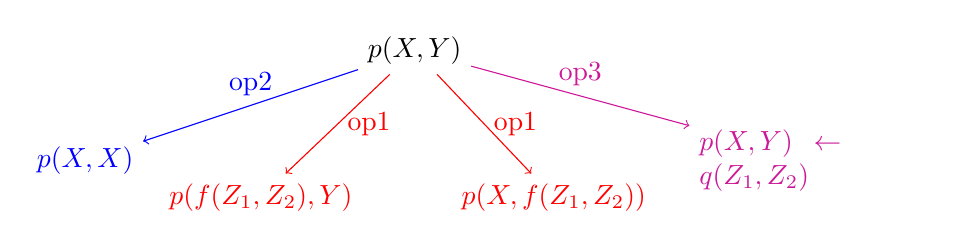
\begin{tikzpicture}[scale=0.93]
				\node (A) at (1.5,1)   {$p(X,Y)$};
				\node (B) at (-3,-0.5) {\color{blue}$p(X,X)$};
				\node (C) at (-0.6,-1) {\color{red}$p(f(Z_1,Z_2), Y)$};
				\node (D) at (3.4,-1)  {\color{red}$p(X,f(Z_1,Z_2))$};
				\node (E)[text width=3cm] at (7,-0.5) {\color{wine-red}$p(X,Y) \leftarrow q(Z_1, Z_2)$};

				\path [->, blue] (A) edge node[above] {op2} (B);
				\path [->, red]  (A) edge node[right] {op1} (C);
				\path [->, red]  (A) edge node[right] {op1} (D);
				\path [->, wine-red]       (A) edge node[above] {op3} (E);
			\end{tikzpicture}
		\end{center}
		\caption{Beispiel für einen Refinement-operator}
		\label{fig:refinement_operator}
	\end{figure}
\end{frame}

\begin{frame}
	\frametitle{Top-Down -- Refinement-Operator}
	\begin{figure}[H]
		\begin{center}
			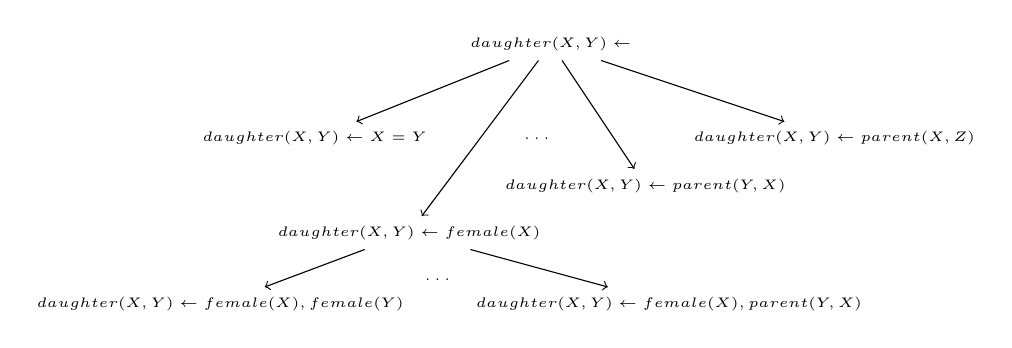
\begin{tikzpicture}[scale=1.2]
				\node[font=\tiny] (A) at (1.5,1) {$daughter(X,Y)\leftarrow$};
				\node[font=\tiny] (B) at (-1,0) {$daughter(X,Y) \leftarrow X = Y$};
				\node[font=\tiny] (C) at (0,-1) {$daughter(X,Y) \leftarrow female(X)$};
				\node[font=\tiny] (D) at (2.5,-0.5) {$daughter(X,Y) \leftarrow parent(Y,X)$};
				\node[font=\tiny] (E) at (4.5,0) {$daughter(X,Y) \leftarrow parent(X, Z)$};
				\node[font=\tiny] (F) at (-2,-1.75) {$daughter(X,Y)\leftarrow female(X), female(Y)$};
				\node[font=\tiny] (G) at (2.75, -1.75) {$daughter(X,Y) \leftarrow female(X), parent(Y,X)$};
				\node[font=\tiny] (X) at (1.35, -0) {$\ldots$};
				\node[font=\tiny] (Y) at (0.3, -1.5) {$\ldots$};

				\path [->] (A) edge node[left] {} (B);
				\path [->] (A) edge node[left] {} (C);
				\path [->] (A) edge node[left] {} (D);
				\path [->] (A) edge node[left] {} (E);
				\path [->] (C) edge node[left] {} (F);
				\path [->] (C) edge node[left] {} (G);
			\end{tikzpicture}
		\end{center}
		\caption{Teil des Refinementgraphs für Familienkonstellation}
		\label{fig:refinement_operator}
	\end{figure}
	\begin{block}{Refinement-Operator}
		$\rho(c) = \{daughter(X, Y) \leftarrow L\}$ mit
		\begin{enumerate}
			\item Argumente von $L$ sind Variablen vom Header
			\item $L$ darf eine neue Variable einführen
		\end{enumerate}
	\end{block}
\end{frame}

\begin{frame}
	\frametitle{Top-Down -- Varianten}
	Wie durchsucht man den Refinementgraph?
	\begin{itemize}
		\item Variante 1: Vollständig (\emph{langsam})
		\item Variante 2: Greedy      (\emph{unvollständig})
	\end{itemize}
	\begin{block}{Verbesserung von Top-Down}
		Verkleinere Suchraum durch Seed
	\end{block}
	\begin{center}
		\begin{tikzpicture}
			\node[font=\tiny] (A) at (1.5,1) {$p(X,Y)$};
				\node[font=\tiny] (B) at (-1,0) {$p(X,X)$};
				\node[font=\tiny] (C) at (0.55,0) {$p(X,Y) \leftarrow r(U)$};
				\node[font=\tiny] (D) at (2.6,0) {$p(X,Y) \leftarrow q(V)$};
				\node[font=\tiny] (E) at (1.5,-2) {$p(X,Y) \leftarrow r(X), q(X), q(Y)$};
				\node[font=\tiny] (X) at (1.75, 0.5) {$\ldots$};
				\node[font=\tiny] (Y) at (0.6, 0.5) {$\ldots$};
				\node[font=\tiny] (B2) at (0.3,-1.3)  {};
				\node[font=\tiny] (C2) at (1.5,-1) {};
				\node[font=\tiny] (D2) at (3,-1.3) {};
				\node[font=\tiny] (B3) at (-1,-1.5) {\ldots};
				\node[font=\tiny] (D3) at (4,-1.5) {\ldots};
				\node[font=\tiny] (X2) at (1, -1.25) {$\ldots$};
				\node[font=\tiny] (Y2) at (2, -1.25) {$\ldots$};

				\path [->] (A) edge node[left] {} (B);
				\path [->] (A) edge node[left] {} (C);
				\path [->] (A) edge node[left] {} (D);
				\path [->] (B2) edge node[left] {} (E);
				\path [->] (C2) edge node[left] {} (E);
				\path [->] (D2) edge node[left] {} (E);
			\begin{scope}[label distance=0mm,]
				\coordinate  (aux1) at ([yshift=-15pt]A);
				\coordinate  (aux2) at ([yshift=+10pt]E);
				\node[regular polygon,regular polygon sides=5,draw, red,fit={(aux1) (aux2)},label=right:{\color{red}\small{Bereich mit Seed}}] {};
			\end{scope}
			%\begin{scope}[label distance=6mm,]
			%	\foreach \i/\label in {1/Label 1,2/Label 2,3/Label 3}
			%	{
			%		  \coordinate  (aux\i) at ([xshift=2cm]t\i);
			%		    \node[inner sep=6pt,rounded corners=6pt,draw,red,fit={(t\i) (b\i)
			%			(aux\i)},label=right:{\color{red}\label}] {};
			%			}
			%\end{scope}
		\end{tikzpicture}
	\end{center}
\end{frame}
